\chapter{Fejlesztői dokumentáció}
\label{ch:implementation}

\section{Use-case diagramok}

\subsection{Kliens use-case diagram}

\begin{figure}[H]
	\centering
	\fbox{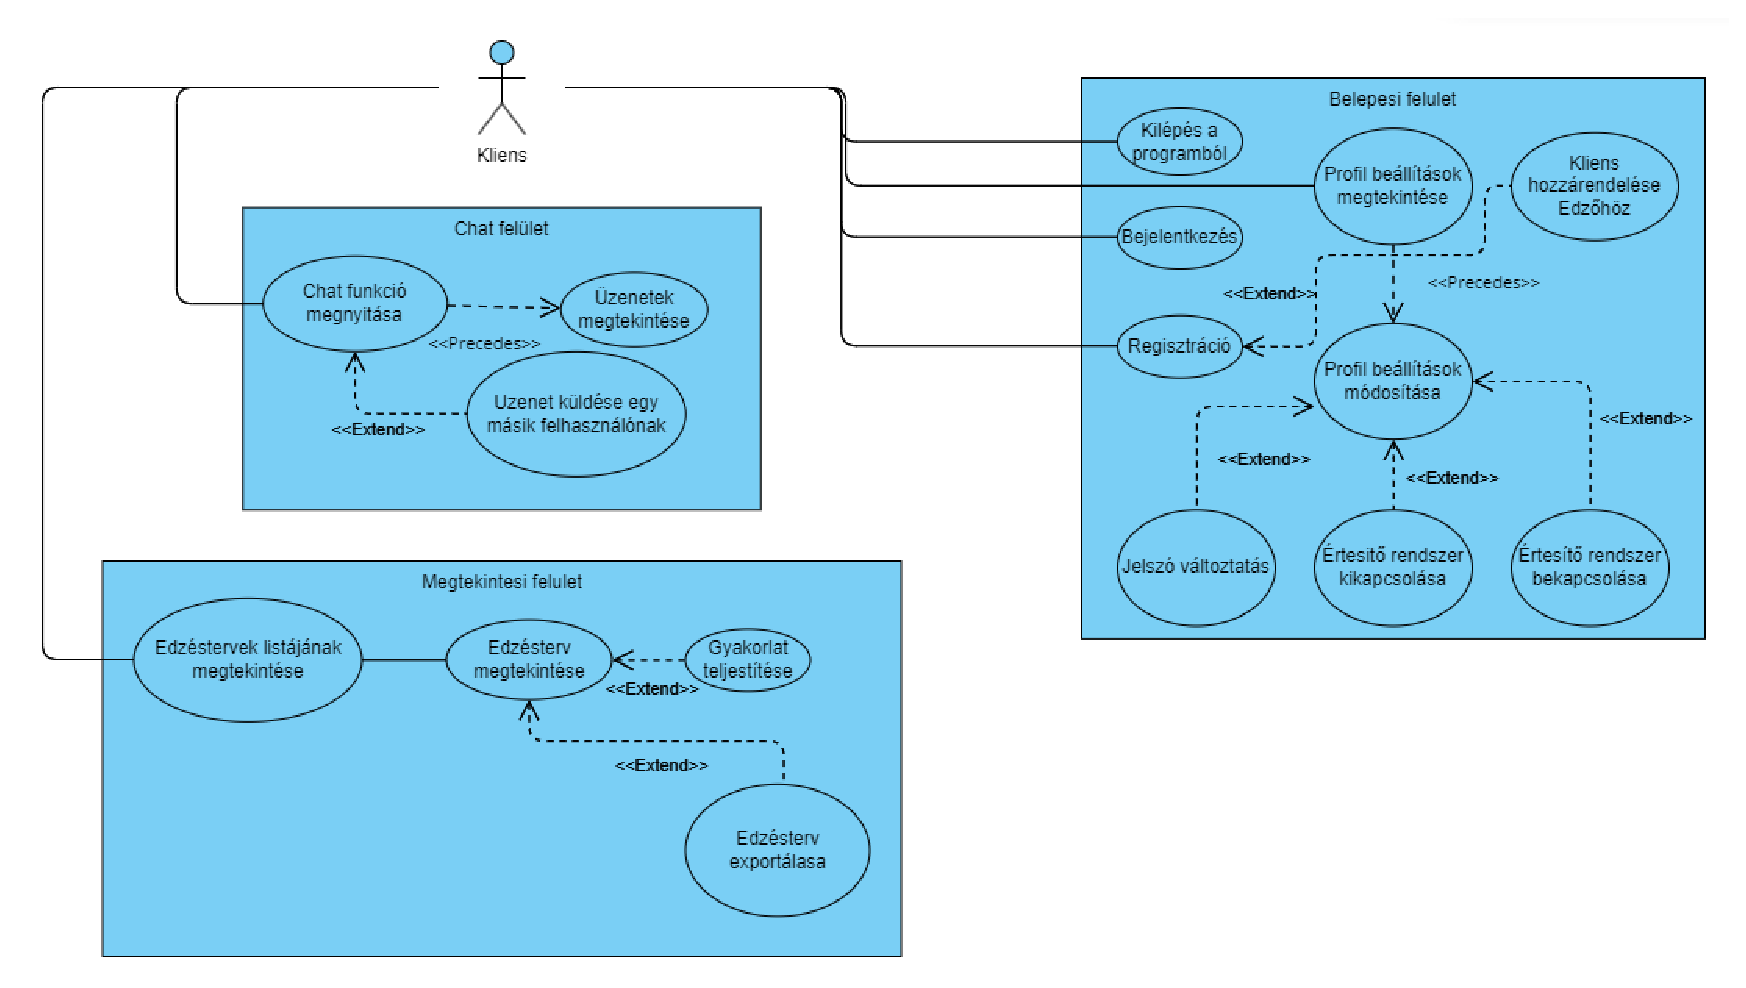
\includegraphics[width=0.97\linewidth]{usecaseclient}}
	\caption{Kliens use-case diagram (készült: Visual Paradigm Online \cite{visualparadigm} nevű programmal)}
	\label{fig:usecaseclient}
\end{figure}

\subsection{Edző use-case diagram}

\begin{figure}[H]
	\centering
	\fbox{\includegraphics[width=0.97\linewidth]{usecasecoach}}
	\caption{Edző use-case diagram (készült: Visual Paradigm Online \cite{visualparadigm} nevű programmal)}
	\label{fig:usecasecoach}
\end{figure}

Edzőknek elérhetőek a kliensek minden fő funkciója, a szerkesztési felület kialakítása hasonló a megtekintési felülethez, kiegészítve szerkesztésre vonatkozó funckiókkal.

\subsection{Adminisztrátor use-case diagram}

\begin{figure}[H]
	\centering
	\fbox{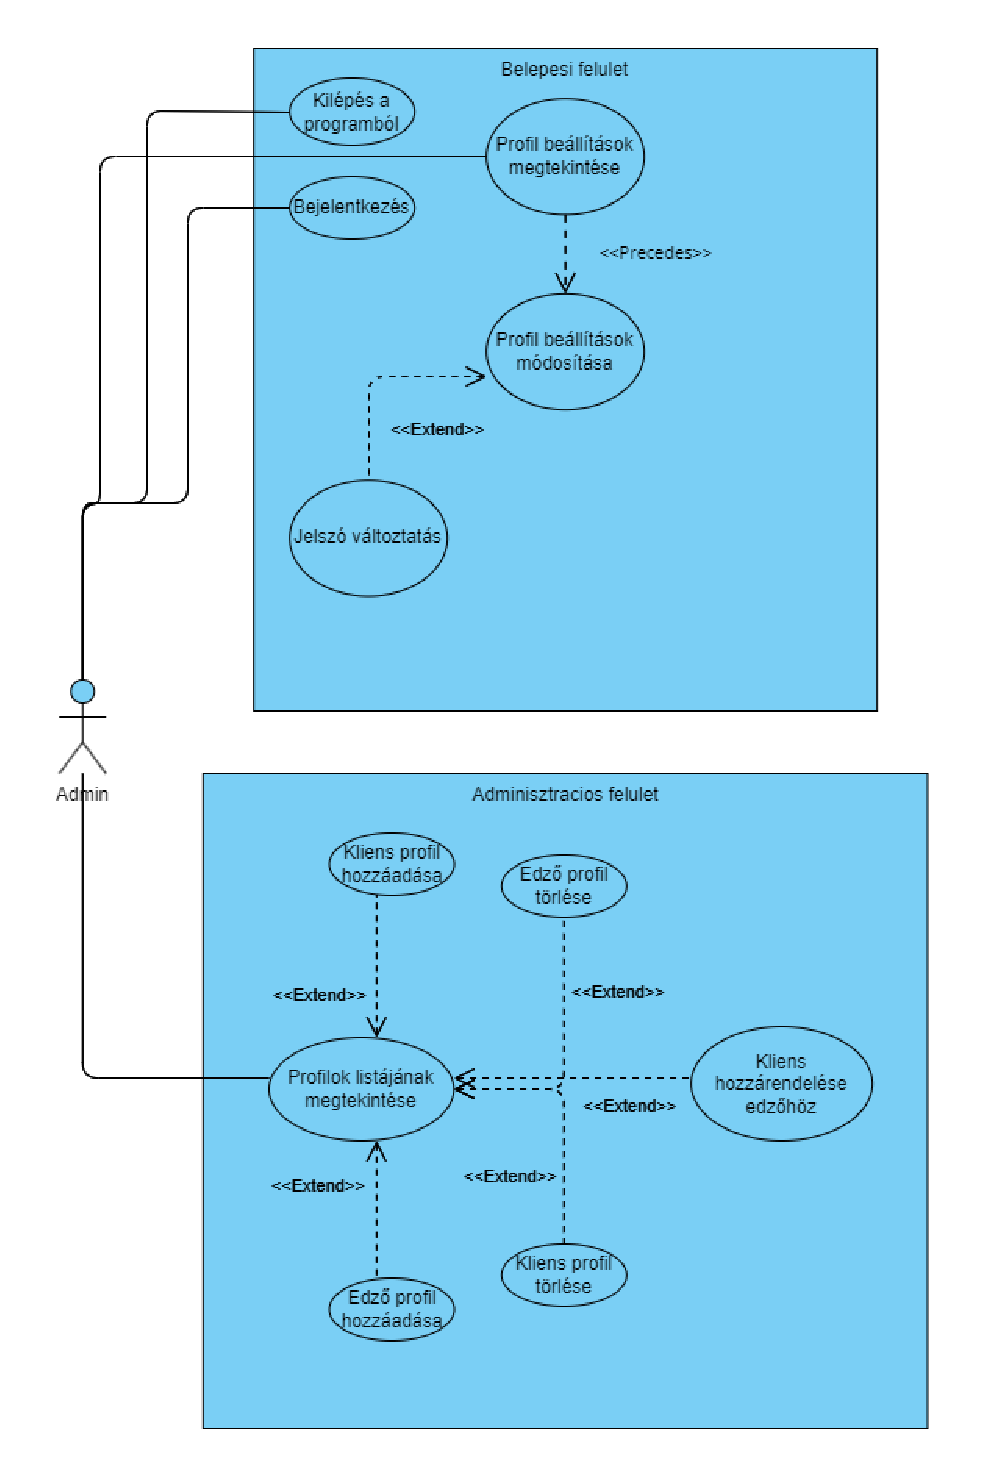
\includegraphics[width=0.8\linewidth]{usecaseadmin}}
	\caption{Adminisztrátor use-case diagram (készült: Visual Paradigm Online \cite{visualparadigm} nevű programmal)}
	\label{fig:usecaseadmin}
\end{figure}

Adminisztrátorként nem elérhetőek a kliens és edző felhasználók funkciói. Egy adminisztrátor csupán a felhasználókat tudja kezelni (törölni, klienseket hozzárendelni edzőkhöz).

\section{User-story táblázatok}

% Latogato userstory

\begin{center}
	\begin{longtable}{ | p{0.06\textwidth} | p{0.2\textwidth} | p{0.1\textwidth} | p{0.54\textwidth} | }
			
			\hline
			\multicolumn{4}{|c|}{\textbf{As a látogató}}
			\\ \hline
			
			\# & Eset & & Leírás
			\\ \hline \hline
			\endfirsthead % első oldal fejléce
			
			\hline
			\# & Eset & & Leírás
			\\ \hline \hline
			\endhead % többi oldal fejléce
			
			\hline
			\endfoot % többi oldal lábléce
			
			\endlastfoot % utolsó oldal lábléce
			
			% Regisztracio

			\multirow{3}{*}{0.1.1} 
			& \multirow{3}{=}{Regisztráció űrlap megnyitása} 
			& GIVEN 
			& Kezdőlap van megjelenítve \\
			\cline{3-4}
			& & WHEN 
			& \emph{"Sign Up"} gombra kattint a felhasználó \\
			\cline{3-4}
			& & THEN 
			& Regisztrációs űrlap megjelenik \\
			\hline

			\multirow{3}{*}{0.1.2} 
			& \multirow{3}{=}{Regisztráció helyes adatokkal} 
			& GIVEN 
			& Regisztrációs űrlap van megjelenítve \\
			\cline{3-4}
			& & WHEN 
			& A felhasználó helyesen tölti ki az űrlapot \\
			\cline{3-4}
			& & THEN 
			& Regisztráció sikeres visszajelző üzenet megjelenik, a bejelentkezett felhasználói kezdőlapok valamelyikére kerülünk \\
			\hline

			\multirow{3}{*}{0.1.3} 
			& \multirow{3}{=}{Regisztráció helytelen adatokkal} 
			& GIVEN 
			& Regisztrációs űrlap van megjelenítve \\
			\cline{3-4}
			& & WHEN 
			& A felhasználó helytelenül tölti ki az űrlapot \\
			\cline{3-4}
			& & THEN 
			& Regisztráció hibaüzenet megjelenik \\
			\hline

			% Login

			\multirow{3}{*}{0.2.1} 
			& \multirow{3}{=}{Bejelentkezés} 
			& GIVEN 
			& Kezdőlap van megjelenítve \\
			\cline{3-4}
			& & WHEN 
			& \emph{"Log In"} gombra kattint a felhasználó \\
			\cline{3-4}
			& & THEN 
			& Bejelentkezés űrlap megjelenik \\
			\hline
			
			\multirow{3}{*}{0.2.2} 
			& \multirow{3}{=}{Bejelentkezés helyes adatokkal} 
			& GIVEN 
			& Bejelentkezés űrlap van megjelenítve \\
			\cline{3-4}
			& & WHEN 
			& A felhasználó helyesen tölti ki az űrlapot \\
			\cline{3-4}
			& & THEN 
			& Bejelentkezés sikeres visszajelző üzenet megjelenik, a bejelentkezett felhasználói kezdőlapok valamelyikére kerülünk \\
			\hline

			\multirow{3}{*}{0.2.3} 
			& \multirow{3}{=}{Regisztráció helytelen adatokkal} 
			& GIVEN 
			& Bejelentkezés űrlap van megjelenítve \\
			\cline{3-4}
			& & WHEN 
			& A felhasználó helytelenül tölti ki az űrlapot \\
			\cline{3-4}
			& & THEN 
			& Bejelentkezés hibaüzenet megjelenik \\
			\hline

			\caption{Látogató user-story táblázat}
			\label{tab:userstorylatogato}       
	\end{longtable}
\end{center}

% Client userstory

\pagebreak

\begin{center}
	\begin{longtable}{ | p{0.07\textwidth} | p{0.2\textwidth} | p{0.1\textwidth} | p{0.53\textwidth} | }
			
			\hline
			\multicolumn{4}{|c|}{\textbf{As a kliens}}
			\\ \hline
			
			\# & Eset & & Leírás
			\\ \hline \hline
			\endfirsthead % első oldal fejléce
			
			\hline
			\# & Eset & & Leírás
			\\ \hline \hline
			\endhead % többi oldal fejléce
			
			\hline
			\endfoot % többi oldal lábléce
			
			\endlastfoot % utolsó oldal lábléce
			
			\multirow{3}{*}{1.0.1} 
			& \multirow{3}{=}{Kliens felhasználó kezdőlap megjelenítése} 
			& GIVEN 
			& A felhasználó sikeresen bejelentkezett \\
			\cline{3-4}
			& & WHEN 
			& Bejelentkezés/regisztráció után, vagy a menüből kiválasztva a kezdőlapon van a felhasználó \\
			\cline{3-4}
			& & THEN 
			& Kliens kezdőlap jelenik meg, rajta a megfelelő gombbal \\
			\hline

			% My cycles page
			
			\multirow{3}{*}{1.1.0} 
			& \multirow{3}{=}{"My Cycles" ciklusok listázó oldal megnyitása} 
			& GIVEN 
			& A felhasználó sikeresen bejelentkezett \\
			\cline{3-4}
			& & WHEN 
			& A kezdőlapon vagy a navigációs menüben a "My Cycles" gombra kattintva \\
			\cline{3-4}
			& & THEN 
			& Ciklusok listázó oldal megjelenik a kliens ciklusaival \\
			\hline

			\multirow{3}{*}{1.1.1} 
			& \multirow{3}{=}{Aktív ciklus megnyitása} 
			& GIVEN 
			& Ciklusok listázó oldala megnyitva \\
			\cline{3-4}
			& & WHEN 
			& Egy aktív ciklusra kattintva \\
			\cline{3-4}
			& & THEN 
			& Megjelenik az edzésterv, a megfelelő módosító gombokkal \\
			\hline

			\multirow{3}{*}{1.1.2} 
			& \multirow{3}{=}{Inakvtív ciklus megnyitása} 
			& GIVEN 
			& Ciklusok listázó oldala megnyitva \\
			\cline{3-4}
			& & WHEN 
			& Egy inaktív ciklusra kattintva \\
			\cline{3-4}
			& & THEN 
			& Megjelenik az edzésterv, nem tudjuk módosítani \\
			\hline

			\multirow{3}{*}{1.1.3} 
			& \multirow{3}{=}{PDF letöltése} 
			& GIVEN 
			& Edzésterv megnyitva \\
			\cline{3-4}
			& & WHEN 
			& "Download PDF" gombra kattintva \\
			\cline{3-4}
			& & THEN 
			& A PDF letöltődik, az adatok rajta helyesek \\
			\hline

			\multirow{3}{*}{1.1.4} 
			& \multirow{3}{=}{Súly módosító űrlap megnyitása} 
			& GIVEN 
			& Edzésterv megnyitva \\
			\cline{3-4}
			& & WHEN 
			& Egyik súly oszlopban lévő ceruza ikonra kattintva \\
			\cline{3-4}
			& & THEN 
			& Súly módosító űrlap megjelenik \\
			\hline

			\multirow{3}{*}{1.1.5} 
			& \multirow{3}{=}{Súly módosítása helyesen} 
			& GIVEN 
			& Súly módosító űrlap megnyitva \\
			\cline{3-4}
			& & WHEN 
			& Beírunk egy pozitív számot, elküldjük \\
			\cline{3-4}
			& & THEN 
			& A beírt érték megjelenik az edzéstervben \\
			\hline

			\multirow{3}{*}{1.1.6} 
			& \multirow{3}{=}{Súly módosítása helytelenül} 
			& GIVEN 
			& Súly módosító űrlap megnyitva \\
			\cline{3-4}
			& & WHEN 
			& Beírunk egy negatív számot, vagy nem írunk be semmit \\
			\cline{3-4}
			& & THEN 
			& Hibaüzenet megjelenik, nem tudjuk elküldeni az űrlapot \\
			\hline

			\multirow{3}{*}{1.1.7} 
			& \multirow{3}{=}{Sorozat/ismétlés /RPE módosító űrlap megnyitása} 
			& GIVEN 
			& Edzésterv megnyitva \\
			\cline{3-4}
			& & WHEN 
			& Nem súly oszlopban lévő ceruza ikonra kattintva \\
			\cline{3-4}
			& & THEN 
			& Sorozat/ismétlés/RPE módosító űrlap megjelenik \\
			\hline

			\multirow{3}{*}{1.1.8} 
			& \multirow{3}{=}{Sorozat/ismétlés /RPE módosítása helyesen} 
			& GIVEN 
			& Sorozat/ismétlés/RPE módosító űrlap megnyitva \\
			\cline{3-4}
			& & WHEN 
			& Beírunk egy pozitív számot, elküldjük \\
			\cline{3-4}
			& & THEN 
			& A beírt érték megjelenik az edzéstervben \\
			\hline

			\multirow{3}{*}{1.1.9} 
			& \multirow{3}{=}{Sorozat/ismétlés /RPE módosítása helytelenül} 
			& GIVEN 
			& Sorozat/ismétlés/RPE módosító űrlap megnyitva \\
			\cline{3-4}
			& & WHEN 
			& Beírunk egy negatív számot, vagy nem írunk be semmit \\
			\cline{3-4}
			& & THEN 
			& Hibaüzenet megjelenik, nem tudjuk elküldeni az űrlapot \\
			\hline



			\multirow{3}{*}{1.1.10} 
			& \multirow{3}{=}{Hetek között lapozás jobbra} 
			& GIVEN 
			& Edzésterv megnyitva \\
			\cline{3-4}
			& & WHEN 
			& A képernyő alján jobb nyílra kattintunk \\
			\cline{3-4}
			& & THEN 
			& Az edzésterv következő hetére váltunk, megjelennek a helyes értékek \\
			\hline

			\multirow{3}{*}{1.1.11} 
			& \multirow{3}{=}{Hetek között lapozás balra} 
			& GIVEN 
			& Edzésterv megnyitva \\
			\cline{3-4}
			& & WHEN 
			& A képernyő alján bal nyílra kattintunk \\
			\cline{3-4}
			& & THEN 
			& Az edzésterv következő hetére váltunk, megjelennek a helyes értékek \\
			\hline

			\multirow{3}{*}{1.1.12} 
			& \multirow{3}{=}{Jobb nyíl gomb inaktív} 
			& GIVEN 
			& Edzésterv megnyitva \\
			\cline{3-4}
			& & WHEN 
			& Az utolsó hétre lapoztunk \\
			\cline{3-4}
			& & THEN 
			& A jobb nyíl gomb inaktív \\
			\hline

			\multirow{3}{*}{1.1.13} 
			& \multirow{3}{=}{Bal nyíl gomb inaktív} 
			& GIVEN 
			& Edzésterv megnyitva \\
			\cline{3-4}
			& & WHEN 
			& Az első hétre lapoztunk \\
			\cline{3-4}
			& & THEN 
			& A bal nyíl gomb inaktív \\
			\hline

			\multirow{3}{*}{1.1.14} 
			& \multirow{3}{=}{Mentés gomb aktív} 
			& GIVEN 
			& Edzésterv megnyitva \\
			\cline{3-4}
			& & WHEN 
			& Nem elmentett adatot tartalmaz \\
			\cline{3-4}
			& & THEN 
			& A mentés gomb aktív \\
			\hline

			\multirow{3}{*}{1.1.15} 
			& \multirow{3}{=}{Mentés gomb inaktív} 
			& GIVEN 
			& Edzésterv megnyitva \\
			\cline{3-4}
			& & WHEN 
			& Nem tartalmaz el nem mentett adatot \\
			\cline{3-4}
			& & THEN 
			& A mentés gomb inaktív \\
			\hline

			\multirow{3}{*}{1.1.16} 
			& \multirow{3}{=}{Edzésterv elmentése} 
			& GIVEN 
			& Edzésterv megnyitva, mentés gomb aktív \\
			\cline{3-4}
			& & WHEN 
			& Mentés gombra kattintunk \\
			\cline{3-4}
			& & THEN 
			& A mentés gomb inaktív lesz, az információ helyesen elmentődik \\
			\hline



			\multirow{3}{*}{1.2.0} 
			& \multirow{3}{=}{Chat oldal megnyitása} 
			& GIVEN 
			& A navigációs menü meg van nyitva \\
			\cline{3-4}
			& & WHEN 
			& A "Chat with coach" gombra kattintva \\
			\cline{3-4}
			& & THEN 
			& A chat oldal jelenik meg, betöltenek az üzenetek és a legfrisebb üzenet a képernyőn van \\
			\hline

			\multirow{3}{*}{1.2.1} 
			& \multirow{3}{=}{Üzenet küldése} 
			& GIVEN 
			& Chat oldal megnyitva \\
			\cline{3-4}
			& & WHEN 
			& Üzenet írása a beviteli mezőbe (nem üres) \\
			\cline{3-4}
			& & THEN 
			& Az üzenet elküldésre kerül, látható mindkét oldal számára \\
			\hline







			\multirow{3}{*}{1.3.0} 
			& \multirow{3}{=}{Profil oldal megnyitása} 
			& GIVEN 
			& A felhasználó sikeresen bejelentkezett \\
			\cline{3-4}
			& & WHEN 
			& A kezdőlapon vagy a navigációs menüben az "Account" gombra kattintva \\
			\cline{3-4}
			& & THEN 
			& Profil oldal megjelenik, rajta a helyes információkkal \\
			\hline

			\multirow{3}{*}{1.3.1} 
			& \multirow{3}{=}{Név módosítása} 
			& GIVEN 
			& Profil oldal megnyitva \\
			\cline{3-4}
			& & WHEN 
			& Beírunk egy új nevet, megadjuk a jelszót és mentés gombra kattintunk \\
			\cline{3-4}
			& & THEN 
			& Uj név mentésre kerül \\
			\hline

			\multirow{3}{*}{1.3.2} 
			& \multirow{3}{=}{Értesítések módosítása} 
			& GIVEN 
			& Profil oldal megnyitva \\
			\cline{3-4}
			& & WHEN 
			& Az értesítések csúszkát a kívánt pozícióba állítjuk, megadjuk a jelszót és mentés gombra kattintunk \\
			\cline{3-4}
			& & THEN 
			& A beállítás mentésre kerül \\
			\hline

			\multirow{3}{*}{1.3.3} 
			& \multirow{3}{=}{Jelszó módosítása} 
			& GIVEN 
			& Profil oldal megnyitva \\
			\cline{3-4}
			& & WHEN 
			& Megadjuk a régi jelszót és az új jelszót, mentés gombra kattintunk \\
			\cline{3-4}
			& & THEN 
			& Az új jelszó mentésre kerül \\
			\hline

			\multirow{3}{*}{1.3.4} 
			& \multirow{3}{=}{Profil beállítás módosítása jelszó megadása nélkül} 
			& GIVEN 
			& Profil oldal megnyitva \\
			\cline{3-4}
			& & WHEN 
			& Módosítunk mezőt, nem adjuk meg a jelszót \\
			\cline{3-4}
			& & THEN 
			& A mentés gomb inaktív
			
			\\
			\hline

			\multirow{3}{*}{1.3.5} 
			& \multirow{3}{=}{Profil beállítás módosítása hibás jelszóval} 
			& GIVEN 
			& Profil oldal megnyitva \\
			\cline{3-4}
			& & WHEN 
			& Módosítunk mezőt, hibás jelszót adunk meg, mentés gombra kattintás \\
			\cline{3-4}
			& & THEN 
			& Rossz jelszó hibaüzenet megjelenik, nem mentődik el a módosítás \\
			\hline

			\caption{Kliens user-story táblázat}
			\label{tab:userstoryclient}       
	\end{longtable}
\end{center}

% Edzo userstory

\pagebreak

\begin{center}
	\begin{longtable}{ | p{0.06\textwidth} | p{0.2\textwidth} | p{0.1\textwidth} | p{0.54\textwidth} | }
			
			\hline
			\multicolumn{4}{|c|}{\textbf{As a edző}}
			\\ \hline
			
			\# & Eset & & Leírás
			\\ \hline \hline
			\endfirsthead % első oldal fejléce
			
			\hline
			\# & Eset & & Leírás
			\\ \hline \hline
			\endhead % többi oldal fejléce
			
			\hline
			\endfoot % többi oldal lábléce
			
			\endlastfoot % utolsó oldal lábléce
			
			% Regisztracio

			\multirow{3}{*}{2.0.1} 
			& \multirow{3}{=}{Edző felhasználó kezdőlap megjelenítése} 
			& GIVEN 
			& A felhasználó sikeresen bejelentkezett \\
			\cline{3-4}
			& & WHEN 
			& Bejelentkezés/regisztráció után, vagy a menüből kiválasztva a kezdőlapon van a felhasználó \\
			\cline{3-4}
			& & THEN 
			& Edző kezdőlap jelenik meg, rajta a megfelelő gombbal \\
			\hline

			\multirow{3}{*}{2.1.1} 
			& \multirow{3}{=}{"My Clients" kliensek listázó oldal megnyitása} 
			& GIVEN 
			& A felhasználó sikeresen bejelentkezett \\
			\cline{3-4}
			& & WHEN 
			& A kezdőlapon vagy a navigációs menüben a
			"My Cycles" gombra kattintva \\
			\cline{3-4}
			& & THEN 
			& Kliensek listázó oldal megjelenik az edző klienseivel \\
			\hline

			\multirow{3}{*}{2.2.1} 
			& \multirow{3}{=}{Chat oldal megnyitása} 
			& GIVEN 
			& A kliensek listázó oldal meg van nyitva \\
			\cline{3-4}
			& & WHEN 
			& Egyik kliensen a chat ikonra kattintva \\
			\cline{3-4}
			& & THEN 
			& Adott klienssel megnyílik a chat oldal, betöltenek az üzenetek és a legfrisebb üzenet a képernyőn van \\
			\hline

			\multirow{3}{*}{2.2.2} 
			& \multirow{3}{=}{Üzenet küldése} 
			& GIVEN 
			& Chat oldal megnyitva \\
			\cline{3-4}
			& & WHEN 
			& Üzenet írása a beviteli mez®be (nem üres) \\
			\cline{3-4}
			& & THEN 
			& Az üzenet elküldésre kerül, látható mindkét
			oldal számára \\
			\hline




			\multirow{3}{*}{2.3.1} 
			& \multirow{3}{=}{Kliens ciklusainak listázó oldal megnyitása} 
			& GIVEN 
			& Kliensek listázó oldal meg van nyitva \\
			\cline{3-4}
			& & WHEN 
			& Egyik kliens cellájára kattintva \\
			\cline{3-4}
			& & THEN 
			& Adott kliens ciklusainak listázó oldala megjelenik, a kliens ciklusaival \\
			\hline

			\multirow{3}{*}{2.3.2} 
			& \multirow{3}{=}{Ciklus törlése}
			& GIVEN 
			& Kliens ciklusainak listázó oldala meg van nyitva \\
			\cline{3-4}
			& & WHEN 
			& Törlés gombra kattintva \\
			\cline{3-4}
			& & THEN 
			& Megerősítés után a ciklus törlésre kerül \\
			\hline

			\multirow{3}{*}{2.3.3} 
			& \multirow{3}{=}{Ciklus aktiválása /deaktiválása} 
			& GIVEN 
			& Kliens ciklusainak listázó oldala meg van nyitva \\
			\cline{3-4}
			& & WHEN 
			& Archiválás gombra kattintva \\
			\cline{3-4}
			& & THEN 
			& Ha aktív volt a ciklus, inaktívvá válik, ha inaktív volt, aktívvá \\
			\hline

			\multirow{3}{*}{2.3.4} 
			& \multirow{3}{=}{Ciklus létrehozása} 
			& GIVEN 
			& Kliens ciklusainak listázó oldala meg van nyitva \\
			\cline{3-4}
			& & WHEN 
			& Kék hátterű plusz gombra kattintva \\
			\cline{3-4}
			& & THEN 
			& Név megadása és űrlap elküldése után az új ciklus az aktív listába kerül \\
			\hline

			\multirow{3}{*}{2.3.5} 
			& \multirow{3}{=}{Aktív ciklus megnyitása} 
			& GIVEN 
			& Kliens ciklusainak listázó oldala meg van nyitva \\
			\cline{3-4}
			& & WHEN 
			& Egy aktív ciklusra kattintva \\
			\cline{3-4}
			& & THEN 
			& Megjelenik az edzésterv, a megfelelő módosító gombokkal \\
			\hline

			\multirow{3}{*}{2.3.6} 
			& \multirow{3}{=}{Inaktív ciklus megnyitása} 
			& GIVEN 
			& Kliens ciklusainak listázó oldala meg van nyitva \\
			\cline{3-4}
			& & WHEN 
			& Egy inaktív ciklusra kattintva \\
			\cline{3-4}
			& & THEN 
			& Megjelenik az edzésterv, nem tudjuk módosítani \\
			\hline

			\multirow{3}{*}{2.3.7} 
			& \multirow{3}{=}{PDF letöltése} 
			& GIVEN 
			& Edzésterv megnyitva \\
			\cline{3-4}
			& & WHEN 
			& "Download PDF" gombra kattintva \\
			\cline{3-4}
			& & THEN 
			& A pDF letöltődik, az adatok rajta helyesek \\
			\hline

			\multirow{3}{*}{2.3.8} 
			& \multirow{3}{=}{Súly módosító űrlap megnyitása} 
			& GIVEN 
			& Edzésterv megnyitva \\
			\cline{3-4}
			& & WHEN 
			& Egyik súly oszlopban lévő ceruza ikonra kattintva \\
			\cline{3-4}
			& & THEN 
			& Súly módosító űrlap megjelenik \\
			\hline

			\multirow{3}{*}{2.3.9} 
			& \multirow{3}{=}{Súly módosítása helyesen} 
			& GIVEN 
			& Súly módosító űrlap megnyitva \\
			\cline{3-4}
			& & WHEN 
			& Beírunk egy pozitív számot, elküldjük \\
			\cline{3-4}
			& & THEN 
			& A beírt érték megjelenik az edzéstervben \\
			\hline

			\multirow{3}{*}{2.3.10} 
			& \multirow{3}{=}{Súly módosítása helytelenül} 
			& GIVEN 
			& Súly módosító űrlap megnyitva \\
			\cline{3-4}
			& & WHEN 
			& Beírunk egy negatív számot, vagy nem írunk be semmit \\
			\cline{3-4}
			& & THEN 
			& Hibaüzenet megjelenik, nem tudjuk elküldeni az űrlapot \\
			\hline

			\multirow{3}{*}{2.3.11} 
			& \multirow{3}{=}{Gyakorlat törlése} 
			& GIVEN 
			& Edzésterv megnyitva \\
			\cline{3-4}
			& & WHEN 
			& Egy gyakorlathoz tartozó törlés ikonra kattintva \\
			\cline{3-4}
			& & THEN 
			& A gyakorlat törlődik az edzéstervből \\
			\hline

			\multirow{3}{*}{2.3.12} 
			& \multirow{3}{=}{Gyakorlat módosítása űrlap megnyitása} 
			& GIVEN 
			& Edzésterv megnyitva \\
			\cline{3-4}
			& & WHEN 
			& Egy gyakorlathoz tartozó, a gyakorlat neve alatt lévő ceruza gombra kattintva \\
			\cline{3-4}
			& & THEN 
			& Gyakorlat módosító űrlap megjelenik a jelenlegi adatokkal \\
			\hline

			\multirow{3}{*}{2.3.13} 
			& \multirow{3}{=}{Gyakorlat módosítása helyesen a módosító űrlappal} 
			& GIVEN 
			& Gyakorlat módosító űrlap megnyitva \\
			\cline{3-4}
			& & WHEN 
			& Módosítunk adatokat a gyakorlaton, nem adunk meg negatív számot, elküldjük az űrlapot \\
			\cline{3-4}
			& & THEN 
			& A gyakorlat frissített adatai láthatóak edzéstervben \\
			\hline

			\multirow{3}{*}{2.3.14} 
			& \multirow{3}{=}{Gyakorlat módosítása helytelenül a módosító űrlappal} 
			& GIVEN 
			& Gyakorlat módosító űrlap megnyitva \\
			\cline{3-4}
			& & WHEN 
			& Módosítunk adatokat a gyakorlaton, megadunk negatív számot \\
			\cline{3-4}
			& & THEN 
			& Nem tudjuk elküldeni az űrlapot, hibaüzenet(ek) megjelen(nek) \\
			\hline

			\multirow{3}{*}{2.3.15} 
			& \multirow{3}{=}{Gyakorlat sorhelyének változtatása lefele} 
			& GIVEN 
			& Edzésterv megnyitva \\
			\cline{3-4}
			& & WHEN 
			& Lefele nyíl gombra kattintva \\
			\cline{3-4}
			& & THEN 
			& A gyakorlat lejjebb kerül a listában egy pozícióval \\
			\hline

			\multirow{3}{*}{2.3.16} 
			& \multirow{3}{=}{Gyakorlat sorhelyének változtatása felfele} 
			& GIVEN 
			& Edzésterv megnyitva \\
			\cline{3-4}
			& & WHEN 
			& Felfele nyíl gombra kattintva \\
			\cline{3-4}
			& & THEN 
			& A gyakorlat feljebb kerül a listában egy pozícióval \\
			\hline

			\multirow{3}{*}{2.3.17} 
			& \multirow{3}{=}{Sorozat/ismétlés /RPE módosító űrlap megnyitása} 
			& GIVEN 
			& Edzésterv megnyitva \\
			\cline{3-4}
			& & WHEN 
			& Sorozat/ismétlés/RPE oszlopban lévő ceruza ikonra kattintva \\
			\cline{3-4}
			& & THEN 
			& Sorozat/ismétlés/RPE módosító űrlap megjelenik \\
			\hline

			\multirow{3}{*}{2.3.18} 
			& \multirow{3}{=}{Sorozat/ismétlés /RPE módosítása} 
			& GIVEN 
			& Sorozat/ismétlés/RPE módosító űrlap meg van nyitva \\
			\cline{3-4}
			& & WHEN 
			& Beírunk egy nem negatív számot és elküldjük az űrlapot \\
			\cline{3-4}
			& & THEN 
			& A megadott értéket látjuk az edzéstervben \\
			\hline

			\multirow{3}{*}{2.3.19} 
			& \multirow{3}{=}{Gyakorlat hozzáadása űrlap megnyitása} 
			& GIVEN 
			& Edzésterv megnyitva \\
			\cline{3-4}
			& & WHEN 
			& Adott napon az utolsó gyakorlat alatt lévő plusz gombra kattintva \\
			\cline{3-4}
			& & THEN 
			& Megjelenik az új gyakorlat űrlap \\
			\hline

			\multirow{3}{*}{2.3.20} 
			& \multirow{3}{=}{Gyakorlat hozzáadása} 
			& GIVEN 
			& Új gyakorlat űrlap megnyitva \\
			\cline{3-4}
			& & WHEN 
			& Minden mező kitöltése nem negatív számokkal és egy helyes gyakorlat névvel, űrlap küldése \\
			\cline{3-4}
			& & THEN 
			& Az új gyakorlat látható az edzéstervben megfelelő adatokkal \\
			\hline

			\multirow{3}{*}{2.3.21} 
			& \multirow{3}{=}{Nap törlése} 
			& GIVEN 
			& Edzésterv megnyitva \\
			\cline{3-4}
			& & WHEN 
			& Adott naphoz tartozó törlés ikonra kattintva \\
			\cline{3-4}
			& & THEN 
			& Nap törlésre kerül az edzéstervből a gyakorlataival együtt \\
			\hline

			\multirow{3}{*}{2.3.22} 
			& \multirow{3}{=}{Hét törlése} 
			& GIVEN 
			& Edzésterv megnyitva \\
			\cline{3-4}
			& & WHEN 
			& Hét számát jelző szöveg alatti törlés ikonra kattintva \\
			\cline{3-4}
			& & THEN 
			& Az adott hét törlésre kerül, nézetbe kerül a soron következő hét \\
			\hline

			\multirow{3}{*}{2.3.23} 
			& \multirow{3}{=}{Hét hozzáadása} 
			& GIVEN 
			& Edzésterv megnyitva \\
			\cline{3-4}
			& & WHEN 
			& Az utolsó hétre lapozunk, a jobb nyíl helyén megjelenő zöld plusz ikonra kattintva \\
			\cline{3-4}
			& & THEN 
			& Új hét adódik hozzá az edzéstervhez \\
			\hline

			\multirow{3}{*}{2.3.24} 
			& \multirow{3}{=}{Nap hozzáadása} 
			& GIVEN 
			& Edzésterv megnyitva \\
			\cline{3-4}
			& & WHEN 
			& A táblázat alsó sorában található plusz ikonra kattintva \\
			\cline{3-4}
			& & THEN 
			& Új nap adódik a táblázathoz \\
			\hline

			\multirow{3}{*}{2.3.25} 
			& \multirow{3}{=}{Edzésterv elmentése} 
			& GIVEN 
			& Edzésterv megnyitva, mentés gomb aktív \\
			\cline{3-4}
			& & WHEN 
			& Mentés gombra kattintva \\
			\cline{3-4}
			& & THEN 
			& A mentés gomb inaktív lesz, az információ helyesen elmentődik \\
			\hline




			\multirow{3}{*}{2.4.1} 
			& \multirow{3}{=}{Profil oldal megnyitása} 
			& GIVEN 
			& A felhasználó sikeresen bejelentkezett \\
			\cline{3-4}
			& & WHEN 
			& A kezdőlapon vagy a navigációs menüben az "Account" gombra kattintva \\
			\cline{3-4}
			& & THEN 
			& Proil oldal megjelenik, rajta a helyes információkkal \\
			\hline

			\multirow{3}{*}{2.4.2} 
			& \multirow{3}{=}{Név módosítása} 
			& GIVEN 
			& Profil oldal megnyitva \\
			\cline{3-4}
			& & WHEN 
			& Beírunk egy új nevet, megadjuk a jelszót és mentés gombra kattintunk \\
			\cline{3-4}
			& & THEN 
			& Uj név mentésre kerül \\
			\hline

			\multirow{3}{*}{2.4.3} 
			& \multirow{3}{=}{Értesítések módosítása} 
			& GIVEN 
			& Profil oldal megnyitva \\
			\cline{3-4}
			& & WHEN 
			& Az értesítések csúszkát a kívánt pozícióba állítjuk, megadjuk a jelszót és mentés gombra kattintunk \\
			\cline{3-4}
			& & THEN 
			& A beállítás mentésre kerül \\
			\hline

			\multirow{3}{*}{2.4.4} 
			& \multirow{3}{=}{Jelszó módosítása} 
			& GIVEN 
			& Profil oldal megnyitva \\
			\cline{3-4}
			& & WHEN 
			& Megadjuk a régi jelszót és az új jelszót, mentés gombra kattintunk \\
			\cline{3-4}
			& & THEN 
			& Az új jelszó mentésre kerül \\
			\hline

			\multirow{3}{*}{2.4.5} 
			& \multirow{3}{=}{Profil beállítás módosítása jelszó megadása nélkül} 
			& GIVEN 
			& Profil oldal megnyitva \\
			\cline{3-4}
			& & WHEN 
			& Módosítunk mezőt, nem adjuk meg a jelszót \\
			\cline{3-4}
			& & THEN 
			& A mentés gomb inaktív
			
			\\
			\hline

			\multirow{3}{*}{2.4.6} 
			& \multirow{3}{=}{Profil beállítás módosítása hibás jelszóval} 
			& GIVEN 
			& Profil oldal megnyitva \\
			\cline{3-4}
			& & WHEN 
			& Módosítunk mezőt, hibás jelszót adunk meg, mentés gombra kattintás \\
			\cline{3-4}
			& & THEN 
			& Rossz jelszó hibaüzenet megjelenik, nem mentődik el a módosítás \\
			\hline

		

			\caption{Edző user-story táblázat}
			\label{tab:userstoryedzo}       
	\end{longtable}
\end{center}


% Admin usecase

\begin{center}
	\begin{longtable}{ | p{0.06\textwidth} | p{0.2\textwidth} | p{0.1\textwidth} | p{0.54\textwidth} | }
			
			\hline
			\multicolumn{4}{|c|}{\textbf{As a adminisztrátor}}
			\\ \hline
			
			\# & Eset & & Leírás
			\\ \hline \hline
			\endfirsthead % első oldal fejléce
			
			\hline
			\# & Eset & & Leírás
			\\ \hline \hline
			\endhead % többi oldal fejléce
			
			\hline
			\endfoot % többi oldal lábléce
			
			\endlastfoot % utolsó oldal lábléce

			\multirow{3}{*}{3.0.1} 
			& \multirow{3}{=}{Admin felhasználó kezdőlap megjelenítése} 
			& GIVEN 
			& A felhasználó sikeresen bejelentkezett \\
			\cline{3-4}
			& & WHEN 
			& Bejelentkezés/regisztráció után, vagy a menüből kiválasztva a kezdőlapon van a felhasználó \\
			\cline{3-4}
			& & THEN 
			& Admin kezdőlap jelenik meg \\
			\hline
			
			\multirow{3}{*}{3.1.1} 
			& \multirow{3}{=}{Felhasználók listájának megtekintése} 
			& GIVEN 
			& A felhasználó sikeresen bejelentkezett \\
			\cline{3-4}
			& & WHEN 
			& Navigációs menüben a \emph{"Manage Users"} gombra kattint a felhasználó \\
			\cline{3-4}
			& & THEN 
			& Felhasználók listázó oldala megjelenik \\
			\hline

			\multirow{3}{*}{3.1.1} 
			& \multirow{3}{=}{Lista szűrése összes felhasználóra} 
			& GIVEN 
			& Felhasználók listázó oldala megnyitva \\
			\cline{3-4}
			& & WHEN 
			& Felső szűrő menüben az \emph{"All"} szűrő kiválasztása \\
			\cline{3-4}
			& & THEN 
			& Az összes regisztrált felhasználót látjuk \\
			\hline

			\multirow{3}{*}{3.1.1} 
			& \multirow{3}{=}{Lista szűrése kliens felhasználókra} 
			& GIVEN 
			& Felhasználók listázó oldala megnyitva \\
			\cline{3-4}
			& & WHEN 
			& Felső szűrő menüben az \emph{"Client"} szűrő kiválasztása \\
			\cline{3-4}
			& & THEN 
			& Az összes kliens felhasználót látjuk \\
			\hline

			\multirow{3}{*}{3.1.1} 
			& \multirow{3}{=}{Lista szűrése edző felhasználókra} 
			& GIVEN 
			& Felhasználók listázó oldala megnyitva \\
			\cline{3-4}
			& & WHEN 
			& Felső szűrő menüben az \emph{"Coach"} szűrő kiválasztása \\
			\cline{3-4}
			& & THEN 
			& Az összes edző felhasználót látjuk \\
			\hline

			\multirow{3}{*}{3.1.1} 
			& \multirow{3}{=}{Lista szűrése admin felhasználókra} 
			& GIVEN 
			& Felhasználók listázó oldala megnyitva \\
			\cline{3-4}
			& & WHEN 
			& Felső szűrő menüben az \emph{"Admin"} szűrő kiválasztása \\
			\cline{3-4}
			& & THEN 
			& Az összes admin felhasználót látjuk \\
			\hline

			\multirow{3}{*}{3.1.1} 
			& \multirow{3}{=}{Felhasználó törlése} 
			& GIVEN 
			& Felhasználók listázó oldala megnyitva \\
			\cline{3-4}
			& & WHEN 
			& Adott felhasználó cellájában a \emph{"Delete User"} gombra kattintva \\
			\cline{3-4}
			& & THEN 
			& A felugró ablak elfogadása után a felhasználó törlésre kerül \\
			\hline

			\multirow{3}{*}{3.1.1} 
			& \multirow{3}{=}{Edző felhasználó klienseinek megtekintése} 
			& GIVEN 
			& Felhasználók listázó oldala megnyitva \\
			\cline{3-4}
			& & WHEN 
			& Egy edző felhasználó cellájában a \emph{"Clients"} fül lenyitása \\
			\cline{3-4}
			& & THEN 
			& Megjelenik az edző összes kliense egy listában \\
			\hline

			\multirow{3}{*}{3.1.1} 
			& \multirow{3}{=}{Kliens törlése edzőtől} 
			& GIVEN 
			& Egy edző felhasználó cellájában a \emph{"Clients"} fül lenyitva \\
			\cline{3-4}
			& & WHEN 
			& Adott kliens cellájában a \emph{"Delete Client"} gombra kattintva \\
			\cline{3-4}
			& & THEN 
			& Kliens hozzárendelése az edzőhöz megszűnik \\
			\hline






			\multirow{3}{*}{2.4.1} 
			& \multirow{3}{=}{Profil oldal megnyitása} 
			& GIVEN 
			& A felhasználó sikeresen bejelentkezett \\
			\cline{3-4}
			& & WHEN 
			& A kezdőlapon vagy a navigációs menüben az "Account" gombra kattintva \\
			\cline{3-4}
			& & THEN 
			& Proil oldal megjelenik, rajta a helyes információkkal \\
			\hline

			\multirow{3}{*}{2.4.2} 
			& \multirow{3}{=}{Név módosítása} 
			& GIVEN 
			& Profil oldal megnyitva \\
			\cline{3-4}
			& & WHEN 
			& Beírunk egy új nevet, megadjuk a jelszót és mentés gombra kattintunk \\
			\cline{3-4}
			& & THEN 
			& Uj név mentésre kerül \\
			\hline

			\multirow{3}{*}{2.4.4} 
			& \multirow{3}{=}{Jelszó módosítása} 
			& GIVEN 
			& Profil oldal megnyitva \\
			\cline{3-4}
			& & WHEN 
			& Megadjuk a régi jelszót és az új jelszót, mentés gombra kattintunk \\
			\cline{3-4}
			& & THEN 
			& Az új jelszó mentésre kerül \\
			\hline

			\multirow{3}{*}{2.4.5} 
			& \multirow{3}{=}{Profil beállítás módosítása jelszó megadása nélkül} 
			& GIVEN 
			& Profil oldal megnyitva \\
			\cline{3-4}
			& & WHEN 
			& Módosítunk mezőt, nem adjuk meg a jelszót \\
			\cline{3-4}
			& & THEN 
			& A mentés gomb inaktív \\
			\hline

			\multirow{3}{*}{2.4.6} 
			& \multirow{3}{=}{Profil beállítás módosítása hibás jelszóval} 
			& GIVEN 
			& Profil oldal megnyitva \\
			\cline{3-4}
			& & WHEN 
			& Módosítunk mezőt, hibás jelszót adunk meg, mentés gombra kattintás \\
			\cline{3-4}
			& & THEN 
			& Rossz jelszó hibaüzenet megjelenik, nem mentődik el a módosítás \\
			\hline

			\caption{Adminisztrátor user-story táblázat}
			\label{tab:userstoryadmin}       
	\end{longtable}
\end{center}

\section{Űrlapokon bekért adatokra vonatkozó követelmények}

\subsubsection{Ciklus/edzésterv oldal}

\begin{itemize}
	\item Gyakorlat neve: Kötelező, maximum 30 karakter
	\item Súly: $x \in \mathbb{N}$, $0 \leq x < 10000$
	\item Sorozatok, ismétlések: Kötelező, $x \in \mathbb{N}$, $0 \leq x < 100$
	\item RPE: Kötelező, listából választott szám $x \in \{5, 6, 7, 8, 8.5, 9, 10\}$
\end{itemize}

\subsubsection{Regisztráció/profil oldal}

\begin{itemize}
	\item Profil név: Kötelező, maximum 20 karakter
	\item Email cím: Kötelező, valid email cím
	\item Jelszó: Kötelező
\end{itemize}

\subsubsection{Chat}

\begin{itemize}
	\item Üzenet hossza: Maximum 255 karakter
\end{itemize}

\pagebreak

\section{Megvalósítás és használt technológiák}

A weboldal fejlesztése során a frontendhez JavaScript alapú React \cite{react} keretrendszert, backendhez pedig NodeJs-t \cite{nodejs} használtam, amely szintén JavaScript alapú.

\bigskip

Vite build eszközt vettem igénybe a lokális fejlesztés megkönnyítése érdekében, amely a frontendhez szükséges .css és script fájlokat előállítja a gyökér könyvtárban található vite.config.js alapján.

\bigskip

A legjelentősebb használt függvénykönyvtárakat a következő alfejezetben fogom részletezni.

\bigskip

\begin{description}
	\item[React verzió:] v18.2.0 (2022. 06. 08.)
	\item[NodeJs verzió:] v20.11.0 (2024. 01. 09.)
\end{description}

\bigskip

A program megvalósítása során az MVC tervezési mintát (\ref{ch:mvc}) követtem (Model, View, Controller).


\subsection{Jelentősebb használt függvénykönyvtárak}

\subsubsection{\underline{Frontend}}

\begin{description}
	\item[Material UI (MUI): \cite{materialui}] A Material UI egy felhasználói felület létrehozását segítő könyvtár. Sok előre megírt komponenst tartalmaz, amelyeket a kódban használni lehet. Komponensei reszponzívak, egyszerűen és globálisan témázhatóak.
	\item[React-Redux Toolkit: \cite{reactredux}] A React-Redux könyvtár a globális állapotkezelést teszi lehetővé reactban. Ez javítja az alkalmazás teljesítményét és fenntarthatóságát, különösen nagyobb projektek esetén. A Redux toolkit pedig egy olyan kiegészítő a React-redux könyvtárhoz, amely kényelmesebb, kifejezőbb módot kínál szintaxis szintjén az állapotkezelésre. Illetve magában foglalja az RTK Query-t, segítségével tudunk API-endpointokat definiálni és használni frontend alkalmazásainkban. 
	\item[React-router-dom: \cite{reactrouterdom}] Lehetővé teszi az útvonalak általi navigációt különböző oldalak közötti kapcsolatok figyelembevételével.
\end{description}

\subsubsection{\underline{Backend}}
\begin{description}
	\item[Express: \cite{express}] Egy keretrendszer, amely lehetővé teszi a HTTP kérések kezelését szerverünkön. Segítségével létrehozhatunk REST API végpontokat, igény szerint kiegészítve middlewarekkel.
	\item[Jsonwebtoken: \cite{jsonwebtoken}] Lehetővé teszi a JWT alkalmazását biztonságos és gyors szerveroldai hitelesítésre és azonosításra.
	\item[Mongoose: \cite{mongoose}] Objektum-modellező könyvtár, NoSQL adatbázisokhoz használt. Ebben a projektben MongoDB-vel van alkalmazva. Ez felel az adatbázisban végrehajtott kereső, módosító műveletek elvégzéséért.
	\item[Nodemailer: \cite{nodemailer}] A Nodemailer egy Node.js könyvtár, amely lehetővé teszi az egyszerű és hatékony e-mail küldést a szerveroldali alkalmazásokból.
\end{description}

\section{Nem funkcionális követelmények}

\begin{itemize}
	\item Hatékonyság: 
	\begin{itemize}
		\item Adatok elérhetősége gyorsan és hatékonyan
		\item Kis erőforrásigény
		\item Gyors válaszidő a lekérdezésekre
	\end{itemize}
	\item Megbízhatóság:
	\begin{itemize}
		\item Helyes használat esetén nem lép fel hiba a programban
		\item Hibás használat esetén nem romlik el a program működése, hibaüzenetekkel érthetően kommunikálva van a hiba oka
	\end{itemize}
	\item Biztonság:
	\begin{itemize}
		\item Alapszintű védelem
	\end{itemize}	
	\item Hordozhatóság:
	\begin{itemize}
		\item Egy áltagos teljesítményű számítógépen a megfelelő böngészőprogramok használata mellett helyes működés
	\end{itemize}
	\item Felhasználhatóság:
	\begin{itemize}
		\item Egyszerű és logikus felhasználói felület, kontextus alapú interfész
	\end{itemize}
\end{itemize}

\pagebreak

\section{MVC architektúra}

\label{ch:mvc}

Az MVC (Model, View, Controller) egy olyan szofterfejlesztési architektúra, amelyet három különálló szoftver rész jellemez. Ezeket az egységeket a következő alfejezetekben fogom részletesen tárgyalni, illetve a hozzájuk tartozó szoftver implementációmat bemutatni.

Ezen architektúra alkalmazásával egy logikusan tagolt és könnyen kezelhető programot tudunk készíteni, áltátható könyvtárstruktúrával.

Programomhoz hozzátartozik ezen felül egy \textbf{Router} is, amely a REST API végpontok kezelésért és a kliens-szerver közötti közvetlen kommunikációért felel. Tulajdonképpen a \textbf{Router} fogja továbbítani a helyes kontrollernek a kapott HTTP kérést.

A REST API végpontokhoz használtam még úgynevezett middlewareket. Ezek a függvények mindig a kontroller hívás előtt futnak le, programomban a felhaszáló hitelesítéséért felelnek. Ezeket a metódusokat is az egyik itt található alfejezetben fogom bemutatni.

\subsection{Model}

A model felelős az alkalmazás üzleti logikájának és adatkezelésének végrehajtásáért. Ide tartoznak az adatbázisból érkező adatok kezelése, az adatok feldolgozása és az üzleti szabályok végrehajtása.

Programomban a model rész a backenden, azaz a szerveroldalon található. NodeJs és Mongoose segítségével van megvalósítva, minden modelhez tartozik egy külön JavaScript modul (Mongoose sémáknak nevezi őket), amelynek létezését a Mongoose függvénykönyvtár előírja. Ezek a modulok fogják tartalmazni az adatbázis szerkezeti leírását:
\begin{itemize}
	\item Milyen típusú mezői vannak egy adatbázis objektumnak,
	\item Milyen esetleges megszorításokkal rendelkeznek,
	\item Definiálhatunk sémánkra statikus (osztályszintű) függvényeket, objektumokra értelmezett függvényeket, illetve például middleware-ként funkcionáló függvényeket is, amelyek minden adott sémához tartozó adatbázis elem módosítása előtt lefutó kódot eredményez.
\end{itemize}

A modellek közötti kapcsolatokat a \ref{fig:model} ábrán látható UML diagramon mutatom be.
Az adatbázis részletesebb leírása a \ref{ch:adatbazis} fejezetben található. 

\begin{figure}[H]
	\centering
	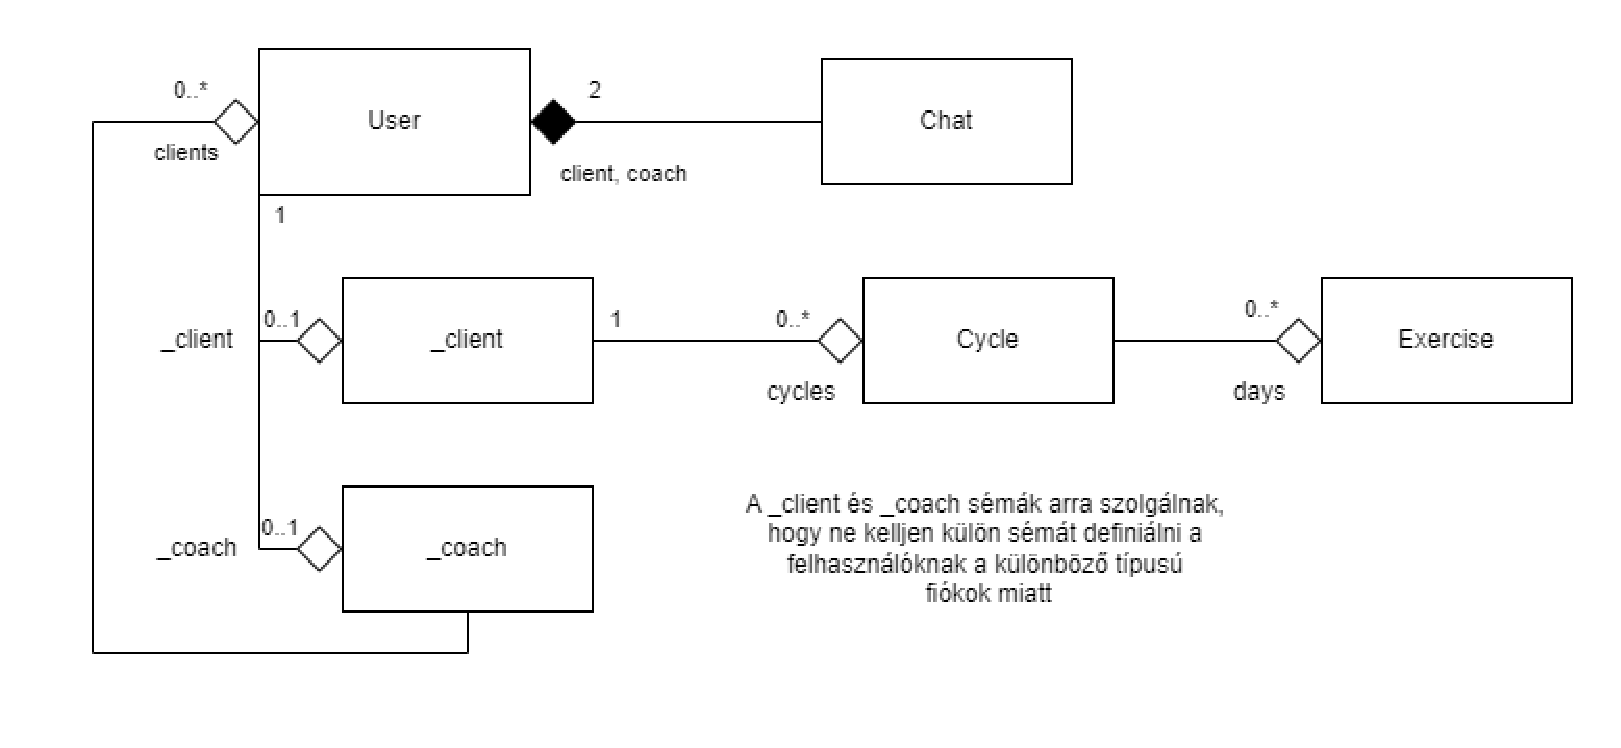
\includegraphics[width=1\linewidth]{model}
	\caption{Modellek (sémák) közötti kapcsolatok}
	\label{fig:model}
\end{figure}

Programomban a "server/schemas" útvonalon érhetőek el az ábrán látható sémák.

\subsection{View}

A view (nézet) felelős az alkalmazás felhasználói felületének megjelenítéséért és a felhasználói interakciók kezeléséért. Ide tartozik az UI elemek létrehozása, elrendezése és formázása, valamint az eseménykezelők hozzárendelése.

A kliensoldali nézetek megjelenítéséért és kezeléséért felelős React komponensek (.jsx kiterjesztésű fájlok, "client/src" útvonalon találhatók) a frontend alkalmazás részét képezik, és közvetlenül kommunikálnak a backenddel HTTP-n keresztül REST API kérések formájában

\subsection{Controller}

Programomban a controller rész a backenden, azaz a szerveroldalon található a "server/controllers" mappában. A Node.js környezetben a routerek és kontrollerek felelősek az útvonalak kezeléséért és az üzleti logika végrehajtásáért. Ezek a kontrollerek az HTTP kéréseket kezelik, és válaszolnak a megfelelő válaszokkal a kliens felé.

A következő alfejezetekben bemutatom a programban lévő kontrollereket, és ezek függvényeit. 

\subsubsection{Általános metódusok}

Ezek a metódusok minden modelhez tartoznak, alapvető adatbázis kezelő utasítások amelyeket a modellekre meghívhatunk.

\begin{itemize}
	\item Model.find(\{\}) - visszaadja az összes modellhez tartozó adatbázis objektumot
	\item Model.find(\{...searchparams\}) - visszaadja a legelső, paraméterekre illeszkedő adatbázis objektumot
	\item Model.save() - elmenti az adatbázisban az adott objektumot
	\item Model.updateOne(\{...searchparams\}, \{...changedattributes\}) - megkeresi a legelső illeszkedő objektumot, majd frissíti a megadott információkkal
	\item Model.deleteOne(\{...serachparams\}) - megkeresi a legelső illeszkedő objektumot és törli az adatbázisból
\end{itemize}

A tobábbiakban A req, res paraméterek a \emph{Request} (kérés) és \emph{Response} (válasz). Mivel a kliensoldal és szerveroldal REST API kérésekkel kommunikál egymással, minden szükséges információ a műveletek végrehajtásához a \emph{Request} paraméterben lesz tárolva JSON formátumban. A \emph{Response} paraméter tartalma pedig visszakerül 

\subsubsection{CycleController}

\begin{figure}[H]
	\centering
	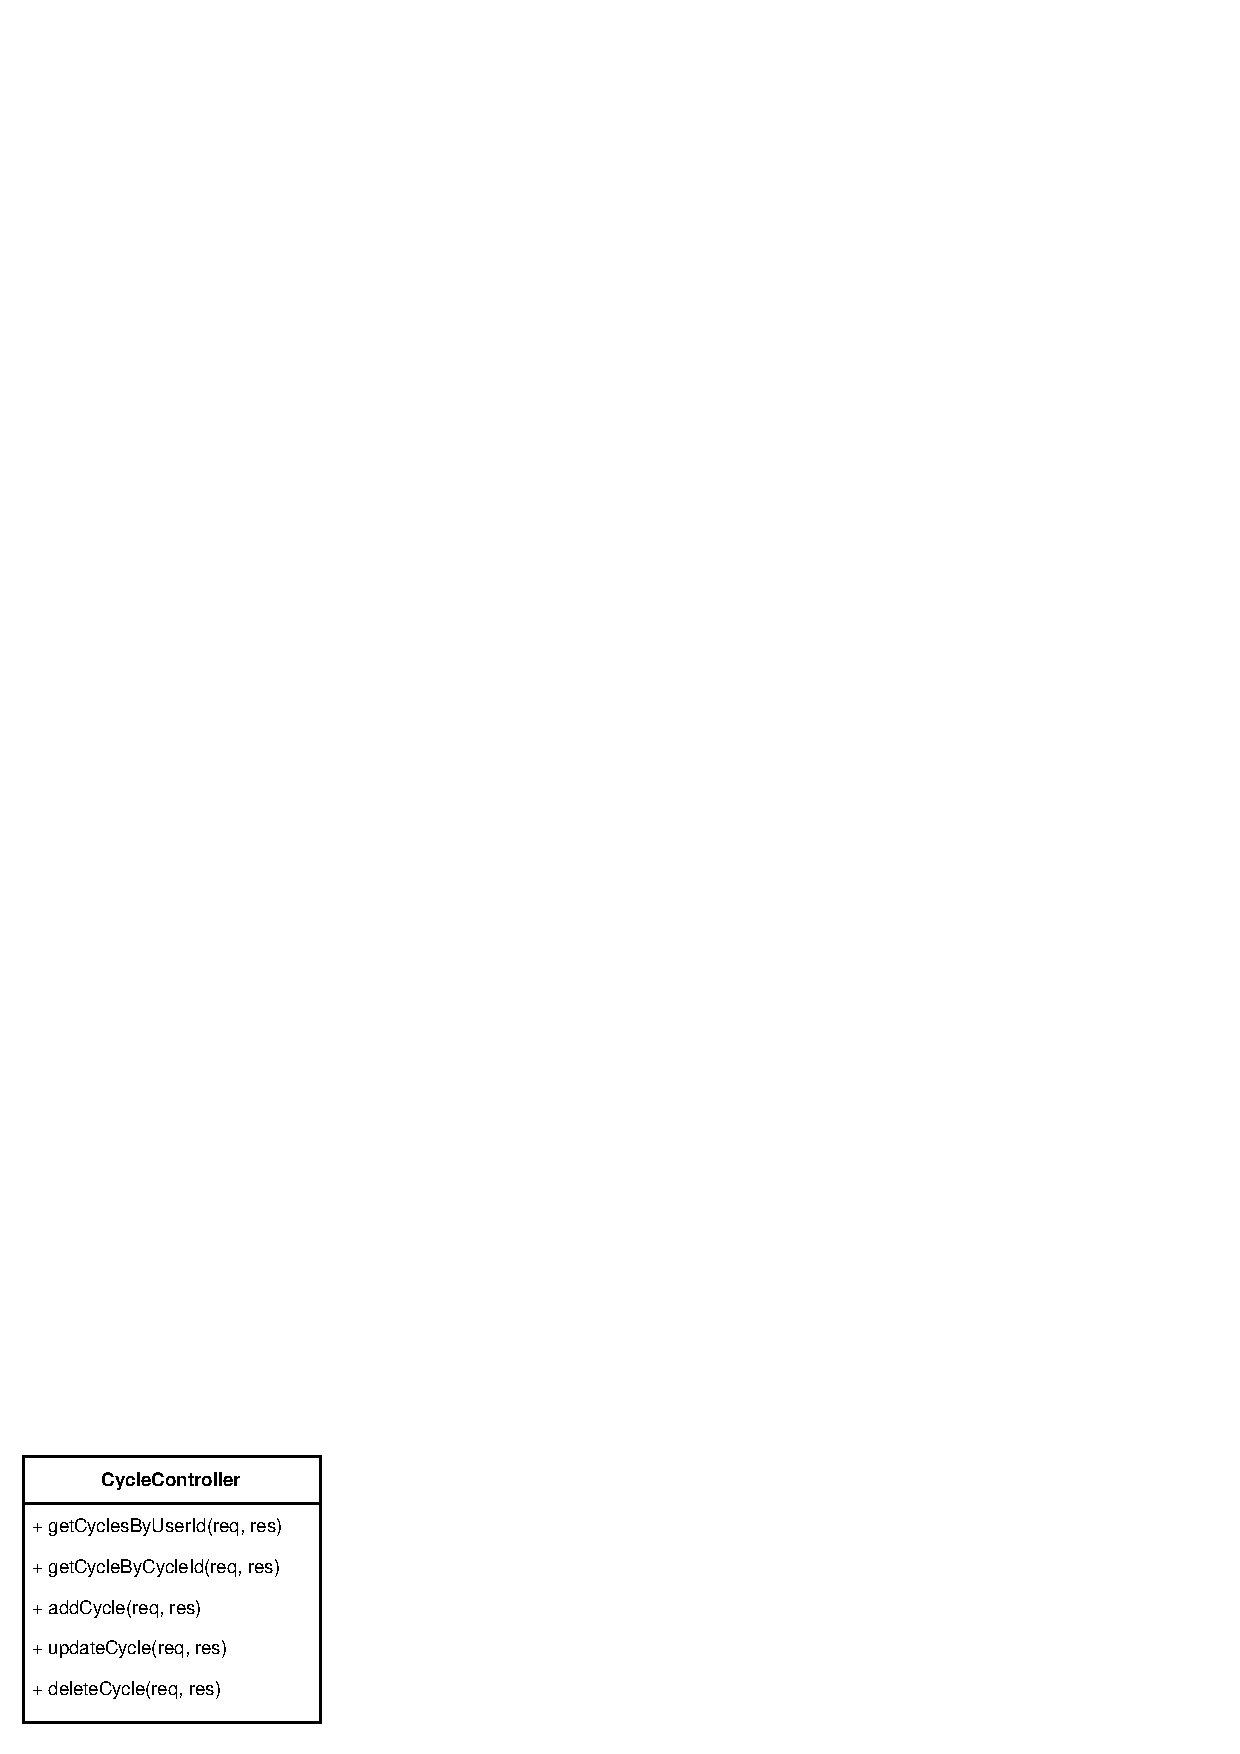
\includegraphics[width=0.4\linewidth]{cyclecontroller}
	\caption{CycleController osztály}
	\label{fig:cyclecontroller}
\end{figure}

A \ref{fig:cyclecontroller} ábrán láthatóak a CycleController osztály metódusai.

\begin{description}
	\item[getCyclesByUserId(req, res):] Visszaadja egy adott felhasználó hoz (ID szerint) tartozó összes ciklus objektumot
	\item[getCycleByCycleId(req, res):] Visszaad egy ciklus objektumot ID alapján
	\item[addCycle(req, res):] A kérésben található JSON-ban tárolt információ alapján létrehoz egy ciklus adatbázis objektumot az adott felhasználóhoz rendelve
	\item[updateCycle(req, res):] Ciklus ID alapján megkeresi a kért objektumot az adatbázisban, és a kérésben JSON-ban tárolt információkra cseréli ki az objektum tartalmát
	\item[deleteCycle(req, res):] Ciklus ID alapján törli a talált objektumot az adatbázisból  
\end{description}

Ha véletlenül egy olyan adatbázis objektumra hívunk meg egy metódust, amelyre nincsen értelmezve, a szerver hibaüzenettel fog visszatérni. Például ha egy edző típusú felhasználóhoz szeretnénk egy új ciklust hozzáadni, a program le fogja kezelni az esetet és hibával tér vissza. 

Ilyen fajta hibakezeléssel mindegyik kontroller rendelkezik, middleware-ként vannak definiálva ezek az ellenőrző és hibakezelő függvények.

\subsubsection{UserController}

\begin{figure}[H]
	\centering
	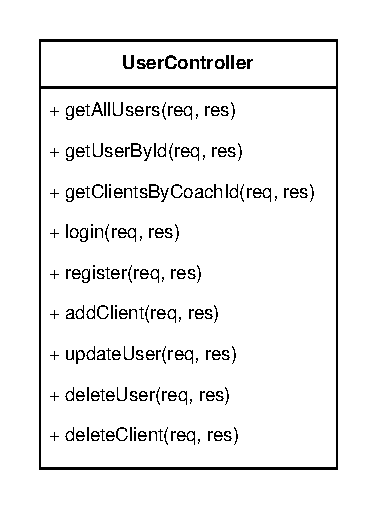
\includegraphics[width=0.4\linewidth]{usercontroller}
	\caption{UserController osztály}
	\label{fig:usercontroller}
\end{figure}

A \ref{fig:usercontroller} ábrán láthatóak a UserController osztályhoz tartozó függvények.

\begin{description}
	\item[getClientsByCoachId(req, res):] Edző objektumnak adja vissza az összes hozzárendelt kliens objektumot
	\item[login(req, res):] Bejelentkezést kezeli, sikeres hitelesítés után egy aláírt JWT tokent küld vissza a kliensnek
	\item[register(req, res):] Sikeres regisztráció után egy aláírt JWT tokent küld vissza, illetve kezeli az edzőhöz való ID alapú hozzárendelést is
	\item[addClient(req, res):] Kliens objektumok edzőhöz való rendelésére szolgál
	\item[deleteUser(req, res):] Töröl egy felhasználót az adatbázisból, ha kliens típusú akkor a hozzá tartozó ciklusokat is törli
	\item[deleteClient(req, res):] Megszüntet egy kliens-edző hozzárendelést
\end{description}

A getAllUsers, getUserById, updateUser metódusokhoz nem szükséges külön magyarázat, ezek a függvények minden fajta User objektumra használhatóak.

\subsubsection{ChatController}

\begin{figure}[H]
	\centering
	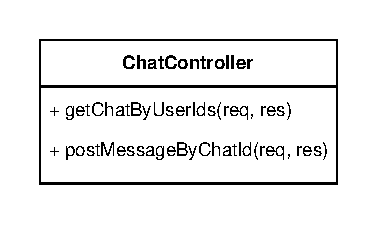
\includegraphics[width=0.4\linewidth]{chatcontroller}
	\caption{ChatController osztály}
	\label{fig:chatcontroller}
\end{figure}

A \ref{fig:chatcontroller} ábrán látható a ChatController osztály metódusai.

\begin{description}
	\item[getChatByUserIds(req, res):] Egy kliens és egy edző közötti chatet keresi meg, a két felhaszáló azonosítójából
	\item[postMessageByChatId(req, res):] Üzenet elküldésére szolgál egy chatben
\end{description}


\subsection{Router}

Ebben az alfejezetben a \textbf{Router} REST API útvonalait fogom felsorolni és leírni a hozzá tartozó kontroller hívást. A \emph{":param"} szöveg mindig egy paramétert jelent az útvonalakban.

\subsubsection{\underline{GET végpontok}}

\begin{description}
	\item[/users] - UserController.getAllUsers
	\item[/users/:id] - UserController.getUserById 
	\item[/users/:id/cycles] - CycleController.getCyclesByUserId
	\item[/users/:id/cycles/:cycleid] - CycleController.getCycleByCycleId
	\item[/users/:id/clients] - UserController.getClientsByCoachId
	\item[/chat/:clientId/:coachId] - ChatController.getChatByUserIds
\end{description}

\subsubsection*{\underline{POST végpontok}}

\begin{description}
	\item[/auth/login] - UserController.login
	\item[/auth/register] - UserController.register
	\item[/users/:id/cycles] -  CycleController.addCycle
	\item[/users/:id/clients] - UserController.addClient
	\item[/chat/:chatId] - ChatController.postMessageByChatId
\end{description}

\subsubsection{\underline{PATCH végpontok}}

\begin{description}
	\item[/users/:id/cycles/:cycleid] - CycleController.updateCycle
	\item[/users/:id] - UserController.updateUser
\end{description}

\subsubsection{\underline{DELETE végpontok}}

\begin{description}
	\item[/users/:id] - UserController.deleteUser
	\item[/users/:id/cycles/:cycleid] - CycleController.deleteCycle
	\item[/users/:id/clients/:clientid] - UserController.deleteClient
\end{description}


\subsection{Middlerwarek}

\begin{itemize}
	\item authMiddleware
	\begin{itemize}
		\item authenticateToken - Ez a függvény felel a JWT tokenek hitelesítéséért, ellenőrzi hogy az aláírás és lejárati időbélyeg valid-e
	\end{itemize}
	\item userTypeMiddleware
	\begin{itemize}
		\item userTypeClient - Ellenőrzi, hogy a kérést küldő felhasználó létezik-e és valóban kliens típusú
		\item userTypeCoach - Ugyanez, edző felhasználóra
		\item userTypeAdmin - Ugyanez, adminisztrátor felhasználóra
		\item isClientIdValid - Ellenőrzi, hogy a kapott ID hivatkozik-e egy kliens objektumra
		\item isCoachIdValid - Ugyanez, edző felhasználóra
	\end{itemize}
\end{itemize}